\scanpage{24}
\unsure{Considerons|Considérons} la partition $\Pi_I^{\unsure{\circ|0}}$ de $X\setminus\bigcup_{\alpha'\in I}E_{\alpha'}$,
% BEGIN C024-M01
\begin{tikzpicture}[x=1pt,y=1pt,baseline=0pt,line cap=round,line join=round]
\path[use as bounding box] (0,-2) rectangle (20,15);
\node[anchor=base west,inner sep=0pt,outer sep=0pt] (soitword) at (0,0) {soit};
\node[anchor=base west,inner sep=0pt,outer sep=0pt] at (1,12) {\unsure{\begin{tikzpicture}[x=1pt,y=1pt,baseline=0pt]\fill (0,0)--(.5,.55)--(1.05,.05)--(.55,-.45)--cycle;\end{tikzpicture}}};
\end{tikzpicture}
% END C024-M01
$S$ l'ens des classes, notées $U_s$ $(s\in S)$.
% BEGIN C024-G02
\unsure{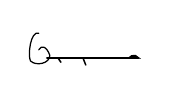
\begin{tikzpicture}[x=1pt,y=1pt,baseline=0pt,line cap=round,line join=round]
\path[use as bounding box] (0,-2) rectangle (43,13);
% Complete states: \deleted{On a} | \deleted{On}. Editorial separators are not manuscript punctuation.
\node[anchor=base west,inner sep=0pt,outer sep=0pt] at (0,0) {\phantom{\deleted{\unsure{On a|On}}}};
\draw[line width=.45pt] (4,11) .. controls (1,12) and (0,3) .. (1,1) .. controls (3,-1) and (8,0) .. (8,3) .. controls (7,6) and (5,7) .. (4,5);
\draw[line width=.8pt] (7,2)--(40,2);
\draw[line width=.55pt] (11,2)--(12,.5) (20,2)--(21,-.5);
\fill (36,2)--(37.5,3.1)--(39,3.2)--(41,1.7)--(39,2)--cycle;
\end{tikzpicture}}
% END C024-G02
Considérons la
% BEGIN C024-G03
\figure{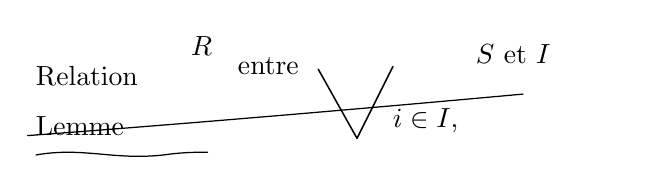
\begin{tikzpicture}[x=1pt,y=1pt,baseline=0pt,line cap=round,line join=round]
\path[use as bounding box] (0,-10) rectangle (215,39);
% Owns the full old and raised lines. Live insertion: Relation R entre S et I.
\node[anchor=base west,inner sep=0pt,outer sep=0pt] at (0,0) {\phantom{\deleted{\uline{Lemme} $\forall i\in I$,}}};
\node[anchor=base west,inner sep=0pt,outer sep=0pt] at (0,22) {\phantom{\inserted{Relation $R$ entre $S$ et $I$}}};
\node[anchor=base west,inner sep=0pt,outer sep=0pt] at (3,0) {Lemme};
\node[anchor=base west,inner sep=0pt,outer sep=0pt] at (3,18) {Relation};
\node[anchor=base west,inner sep=0pt,outer sep=0pt] at (59,29) {$R$};
\node[anchor=base west,inner sep=0pt,outer sep=0pt] at (76,22) {entre};
\node[anchor=base west,inner sep=0pt,outer sep=0pt] at (162,26) {$S$ et $I$};
\draw[line width=.55pt] (105,24)--(119,-1)--(132,25);
\node[anchor=base west,inner sep=0pt,outer sep=0pt] at (132,3) {$i\in I$,};
\draw[line width=.45pt] (0,0) .. controls (67,5) and (135,11) .. (179,15);
\draw[line width=.45pt] (3,-7) .. controls (20,-4) and (31,-9) .. (49,-7) .. controls (56,-6) and (61,-6) .. (65,-6);
% The long cancellation run also crosses the old forall body. No second generic strike is printed.
\end{tikzpicture}}
% END C024-G03
\[
% BEGIN C024-G04
\unsure{\begin{tikzpicture}[x=1pt,y=1pt,baseline=0pt,line cap=round,line join=round]
\path[use as bounding box] (-2,-8) rectangle (20,21);
% Complete states: \deleted{U}(s | \deleted{E}(s. Both own the live opening parenthesis and s once.
\node[anchor=base west,inner sep=0pt,outer sep=0pt] at (0,0) {$\phantom{\deleted{\unsure{U|E}}(s}$};
\draw[line width=.45pt] (0,9) .. controls (-1,16) and (2,17) .. (3,10)--(3,-1) .. controls (4,-4) and (7,-3) .. (8,0)--(8,12);
\draw[line width=.45pt] (2,11) .. controls (4,16) and (6,17) .. (7,14) (7,11) .. controls (9,16) and (11,15) .. (12,14);
\draw[line width=.6pt] (3,10)--(9,12) (3,1)--(9,10) (4,-1)--(8,9) (3,2)--(9,2);
\draw[line width=.45pt] (4,13) .. controls (1,7) and (1,-3) .. (12,-7);
\node[anchor=base west,inner sep=0pt,outer sep=0pt] at (10,-1) {$s$};
% BEGIN C024-M02
\node[anchor=base west,inner sep=0pt,outer sep=0pt] at (1,17) {\unsure{\begin{tikzpicture}[x=1pt,y=1pt,baseline=0pt]\fill (0,0)--(.65,.5)--(1,.05)--(.35,-.4)--cycle;\end{tikzpicture}}};
% END C024-M02
\end{tikzpicture}}
% END C024-G04
,i)\in R\quad
% BEGIN C024-G05
\begin{tikzpicture}[x=1pt,y=1pt,baseline=0pt,line cap=round,line join=round]
\path[use as bounding box] (0,-4) rectangle (34,16);
\node[anchor=base west,inner sep=0pt,outer sep=0pt] at (8,7) {def};
\node[anchor=base west,inner sep=0pt,outer sep=0pt] at (0,0) {$\phantom{\overset{\text{def}}{\Longleftrightarrow}}$};
\draw[line width=.5pt] (6,5) .. controls (2,5) and (0,1) .. (0,0) .. controls (0,-2) and (3,-2) .. (5,-2)--(31,-.5);
\draw[line width=.5pt] (1,1)--(29,1);
\draw[line width=.6pt] (29,1)--(32,-.8) .. controls (33,-1.8) and (31,-2.5) .. (30,-2.6);
\end{tikzpicture}
% END C024-G05
\quad \overline{U_s}\cap E_i\ne\varnothing.
\]

\uline{Lemme} Cette relation fait de $
% BEGIN C024-G06
\unsure{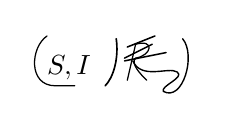
\begin{tikzpicture}[x=1pt,y=1pt,baseline=0pt,line cap=round,line join=round]
\path[use as bounding box] (-2,-9) rectangle (60,17);
% Complete states: (S,I)\deleted{R}) | (S,I\deleted{)},R). Pipes are editorial alternatives.
\node[anchor=base west,inner sep=0pt,outer sep=0pt] at (0,0) {$\phantom{\unsure{(S,I)\deleted{R})|(S,I\deleted{)},R)}}$};
\node[anchor=base west,inner sep=0pt,outer sep=0pt] at (5,0) {$S,I$};
\draw[line width=.45pt] (5,14) .. controls (-1,10) and (-2,-4) .. (8,-4)--(15,-4);
\draw[line width=.6pt] (30,13) .. controls (31,6) and (29,-1) .. (26,-4);
\draw[line width=.45pt] (34,-2)--(37,11) .. controls (44,13) and (43,7) .. (37,6) .. controls (35,4) and (39,0) .. (41,-2);
\draw[line width=.55pt] (34,10)--(44,14) (33,6)--(43,11) (33,5)--(48,8);
\draw[line width=.5pt] (36,5) .. controls (39,-2) and (49,3) .. (52,1) .. controls (55,-1) and (46,-4) .. (47,-6) .. controls (54,-10) and (59,7) .. (54,13);
\end{tikzpicture}}
% END C024-G06
$
% BEGIN C024-G07
\figure{\begin{tikzpicture}[x=1pt,y=1pt,baseline=0pt,line cap=round,line join=round]
\path[use as bounding box] (-19,-61) rectangle (250,20);
\node[anchor=base west,inner sep=0pt,outer sep=0pt] at (0,0) {un graphe strict ayant $S$ comme};
\node[anchor=base west,inner sep=0pt,outer sep=0pt] at (0,-18) {\unsure{ens de|ens des} sommets, $I$ comme ens.};
\node[anchor=base west,inner sep=0pt,outer sep=0pt] at (0,-36) {d'\unsure{aretes|arêtes|arètes}.)};
\node[anchor=base west,inner sep=0pt,outer sep=0pt] at (90,-36) {\rlap{Cette relation}\phantom{\deleted{Cette relation}}};
\draw[line width=.45pt] (88,-33)--(165,-29);
\node[anchor=base west,inner sep=0pt,outer sep=0pt] at (171,-36) {
% BEGIN C024-G08
\unsure{\begin{tikzpicture}[x=1pt,y=1pt,baseline=0pt,line cap=round,line join=round]
\path[use as bounding box] (0,-2) rectangle (21,20);
% Complete word candidates: Le | Ce. Main body and detached upper run stay together.
\node[anchor=base west,inner sep=0pt,outer sep=0pt] at (0,0) {\phantom{\unsure{Le|Ce}}};
\draw[line width=.55pt] (0,13)--(1,1)--(7,1) .. controls (9,-.2) and (11,.4) .. (13,2.8) .. controls (12,1) and (15,.4) .. (19,1.4);
\draw[line width=1pt] (2,12)--(2,14)--(5,17)--(7,16.6)--(9,17.5);
\end{tikzpicture}}
% END C024-G08
};
\node[anchor=base west,inner sep=0pt,outer sep=0pt] at (195,-36) {graphe};
\node[anchor=base west,inner sep=0pt,outer sep=0pt] at (0,-54) {est un \uline{arbre}};
\draw[line width=.5pt] (-8,12) .. controls (-6,15) and (-6,6) .. (-7,0) .. controls (-8,-14) and (-6,-34) .. (-6,-58);
\draw[line width=.3pt] (-8,12) .. controls (-9,7) and (-9,7) .. (-9,5);
% BEGIN C024-M03
\node[anchor=base west,inner sep=0pt,outer sep=0pt] at (-16,-9) {\unsure{\begin{tikzpicture}[x=1pt,y=1pt,baseline=0pt]\draw[gray,line width=.3pt] (0,0)--(.6,2.2);\draw[gray,line width=.2pt] (-.3,-.7)--(-.15,-.3);\end{tikzpicture}}};
% END C024-M03
\end{tikzpicture}}
% END C024-G07

\unsure{le|Le}
% BEGIN C024-M04
\begin{tikzpicture}[x=1pt,y=1pt,baseline=0pt,line cap=round,line join=round]
\path[use as bounding box] (-6,-11) rectangle (19,10);
\node[anchor=base west,inner sep=0pt,outer sep=0pt] at (0,0) {fait};
\node[anchor=base west,inner sep=0pt,outer sep=0pt] at (-3,-9) {\unsure{\begin{tikzpicture}[x=1pt,y=1pt,baseline=0pt]\draw[gray!45,line width=.25pt] (1,7) .. controls (4,4) and (3,1) .. (0,0)--(-2,0);\end{tikzpicture}}};
\end{tikzpicture}
% END C024-M04
% BEGIN C024-G10
\unsure{\begin{tikzpicture}[x=1pt,y=1pt,baseline=0pt,line cap=round,line join=round]
\path[use as bounding box] (-2,-17) rectangle (49,14);
% Complete phrase candidates: qu'on a | qu'on followed by an unassigned point.
% The final point's a/independent-mark question does not remove the whole-phrase qualification.
\node[anchor=base west,inner sep=0pt,outer sep=0pt] at (0,0) {\phantom{\unsure{qu'on a|qu'on $\mathord{\cdot}$}}};
\draw[line width=.4pt] (1,2) .. controls (-2,9) and (1,10) .. (4,5) .. controls (4,2) and (0,1) .. (1,2);
\draw[line width=.35pt] (4,5) .. controls (5,-2) and (7,-12) .. (8,-15) .. controls (7,-16) and (6,-15) .. (6,-14);
\draw[line width=.45pt] (4,5)--(7,8)--(8,7)--(19,7)--(20,11)--(22,9);
\draw[line width=.35pt] (25,7)--(35,7);
\fill (44,7.5) .. controls (44,8.4) and (45.4,8.7) .. (46,8.2)--(45.5,7.4)--cycle;
\end{tikzpicture}}
% END C024-G10
un graphe strict signifie que a) $\forall i\in I$,
% BEGIN C024-G11
\begin{tikzpicture}[x=1pt,y=1pt,baseline=0pt,line cap=round,line join=round]
\path[use as bounding box] (0,-7) rectangle (89,18);
% Complete states: Il \deleted{existe} y a | Il \deleted{ex} y a.
\node[anchor=base west,inner sep=0pt,outer sep=0pt] at (0,0) {\phantom{Il \deleted{\unsure{existe|ex}} y a}};
\draw[line width=.5pt] (1,4)--(3,1)--(5,0)--(7,1) (0,13)--(6,13)--(6,10);
\draw[line width=.4pt] (3,5)--(3,10);
\draw[line width=.45pt] (9,5) .. controls (12,7) and (16,14) .. (14,15) .. controls (10,15) and (11,0) .. (18,0);
\node[anchor=base west,inner sep=0pt,outer sep=0pt] at (20,0) {\unsure{\begin{tikzpicture}[x=1pt,y=1pt,baseline=0pt,line cap=round,line join=round]
\node[anchor=base west,inner sep=0pt,outer sep=0pt] at (0,0) {\phantom{\deleted{\unsure{existe|ex}}}};
\draw[line width=.45pt] (0,2)--(1,0)--(5,.6)--(6,2)--(7,0)--(12,0)--(13,2)--(14,0);
\draw[line width=.7pt] (0,.5)--(36,.5) .. controls (39,0) and (40,2) .. (40,7);
\draw[line width=.45pt] (18,.5)--(20,-2);
\end{tikzpicture}}};
\node[anchor=base west,inner sep=0pt,outer sep=0pt] at (65,0) {y};
% Pale entrance to a is retained once and locally qualified; a remains a live reading.
\node[anchor=base west,inner sep=0pt,outer sep=0pt] at (77,0) {\phantom{a}};
\node[anchor=base west,inner sep=0pt,outer sep=0pt] at (75,0) {\unsure{\begin{tikzpicture}[x=1pt,y=1pt,baseline=0pt]\draw[gray!65,line width=.25pt] (0,-1)--(5,1.5);\end{tikzpicture}}};
\draw[line width=.5pt] (82,2) .. controls (77,1) and (78,-1) .. (84,0);
\end{tikzpicture}
% END C024-G11
exactement deux $U_s$ tels que $\overline{U_s}\cap E_i\ne\varnothing$, et b) $i$ est caractérisé par \unsure{l'ens|l'une} de ces deux $U_s$.

\unsure{Soient|Soit} $
% BEGIN C024-S01
\begin{tikzpicture}[x=1pt,y=1pt,baseline=0pt,line cap=round,line join=round]
\path[use as bounding box] (0,-5) rectangle (24,19);
% Complete reading Sigma_i^+; detached-head role remains head/retrace or independent upper-run.
\node[anchor=base west,inner sep=0pt,outer sep=0pt] at (0,0) {$\phantom{\Sigma_i^+}$};
\node[anchor=base west,inner sep=0pt,outer sep=0pt] at (0,0) {\unsure{\begin{tikzpicture}[x=1pt,y=1pt,baseline=0pt,line cap=round,line join=round]
\draw[line width=.5pt] (2,12)--(1.6,14)--(5,15)--(13,15);
\draw[gray!65,line width=.25pt] (0,11.3)--(2,11.2);
\draw[line width=.45pt] (3,11)--(10,10) .. controls (12,9) and (8,6) .. (1,1)--(15,1.3);
\draw[line width=.45pt] (18,4)--(18,-2);
\fill (18,6) circle (.45pt);
\draw[line width=.6pt] (19.5,16)--(23,16) (21.2,14)--(21.2,18);
\end{tikzpicture}}};
\end{tikzpicture}
% END C024-S01
,
% BEGIN C024-S02
\begin{tikzpicture}[x=1pt,y=1pt,baseline=0pt,line cap=round,line join=round]
\path[use as bounding box] (0,-5) rectangle (24,19);
% Complete locally qualified reading Sigma_i^-; head role remains recorded though first occurrence prints the recurring qualifier.
\node[anchor=base west,inner sep=0pt,outer sep=0pt] at (0,0) {$\phantom{\Sigma_i^-}$};
\draw[line width=.5pt] (2,15)--(11,15.5);
\draw[line width=.3pt] (0,12.8)--(8,11.5);
\draw[line width=.45pt] (9,11) .. controls (11,9) and (4,4) .. (1,1)--(12,1) .. controls (14,1) and (14,-1) .. (14,-2);
\node[anchor=base west,inner sep=0pt,outer sep=0pt] at (16,1) {\unsure{\begin{tikzpicture}[x=1pt,y=1pt,baseline=0pt]\draw[line width=.5pt] (0,4)--(.3,1.2)--(0,0);\end{tikzpicture}}};
\draw[line width=.5pt] (19,15)--(23,15);
\end{tikzpicture}
% END C024-S02
$ les deux comp. \unsure{connexes|conn} de $X\setminus E_i$, alors a) se précise en : il y a \unsure{exactemt|exactement} \uline{un} $
% BEGIN C024-U01
\begin{tikzpicture}[x=1pt,y=1pt,baseline=0pt,line cap=round,line join=round]
\path[use as bounding box] (0,-8) rectangle (24,15);
% Complete candidates U_{s_+} | U_{s_-}; plus remains primary at this physical sign.
\node[anchor=base west,inner sep=0pt,outer sep=0pt] at (0,0) {$U_s\phantom{_{\unsure{+|-}}}$};
\node[anchor=base west,inner sep=0pt,outer sep=0pt] at (15,-6) {\unsure{\begin{tikzpicture}[x=1pt,y=1pt,baseline=0pt]\fill (0,0)--(0,2.5)--(1.3,3.6)--(2.5,3.5)--(2.7,4)--(3.4,3.5)--(5.7,3.5)--(6,2.4)--(4.7,1.9)--(5.7,1.7)--(5.7,.5)--(3,.3)--(0,0)--cycle;\end{tikzpicture}}};
% BEGIN C024-M06
\node[anchor=base west,inner sep=0pt,outer sep=0pt] at (17,0) {\unsure{\begin{tikzpicture}[x=1pt,y=1pt,baseline=0pt]\draw[gray!55,line width=.3pt] (0,1)--(.4,2);\fill[gray!70] (1.6,1.5) circle (.18pt);\end{tikzpicture}}};
% END C024-M06
\end{tikzpicture}
% END C024-U01
$ contenu dans $
% BEGIN C024-S03
\begin{tikzpicture}[x=1pt,y=1pt,baseline=0pt,line cap=round,line join=round]
\path[use as bounding box] (0,-2) rectangle (29,20);
% Complete candidates Sigma_i^- | Sigma_i^+; minus primary at this local solid raised mark.
\node[anchor=base west,inner sep=0pt,outer sep=0pt] at (0,0) {$\phantom{\Sigma_i^{\unsure{-|+}}}$};
\draw[line width=.5pt] (0,15)--(14,15.3);
\draw[line width=.45pt] (5,15) .. controls (12,13) and (11,12) .. (7,10) .. controls (3,7) and (0,5) .. (0,4)--(14,4) .. controls (15,4) and (15,2) .. (15,1);
\draw[line width=.5pt] (17,10)--(16.8,6.5);
\node[anchor=base west,inner sep=0pt,outer sep=0pt] at (21,14) {\unsure{\begin{tikzpicture}[x=1pt,y=1pt,baseline=0pt]\fill (0,0)--(-.3,1)--(.4,2.7)--(2,2.8)--(2.5,3.2)--(3.4,2.8)--(4.8,2.8)--(5.7,1.8)--(5.7,.1)--cycle;\end{tikzpicture}}};
\end{tikzpicture}
% END C024-S03
$ tel que $
% BEGIN C024-U02
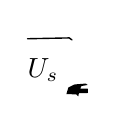
\begin{tikzpicture}[x=1pt,y=1pt,baseline=0pt,line cap=round,line join=round]
\path[use as bounding box] (0,-8) rectangle (25,18);
% Complete local candidates \overline{U_{s_+}} | \overline{U_{s_-}}. Plus primary; later recurring sign printed without a second visible qualifier.
\node[anchor=base west,inner sep=0pt,outer sep=0pt] at (0,0) {$U_s\phantom{_{\unsure{+|-}}}$};
\draw[line width=.5pt] (0,14)--(15,14.3)--(16,13.6);
\fill (14,-6)--(14.7,-3.6)--(17,-2.5)--(21,-2.2)--(21.7,-2.7)--(19.4,-3.1)--(19,-4)--(21.7,-4)--(21.8,-5.6)--(18.5,-5.7)--(18.3,-6.8)--(17.5,-6.1)--cycle;
\end{tikzpicture}
% END C024-U02
\cap
% BEGIN C024-E01

\begin{tikzpicture}[x=1pt,y=1pt,baseline=0pt,line cap=round,line join=round]
\path[use as bounding box] (0,-4) rectangle (25,18);
\node[anchor=base west,inner sep=0pt,outer sep=0pt] at (0,0) {$\phantom{E_i}$};
\draw[line width=.45pt] (0,13.8) .. controls (4,15) and (6,15.5) .. (9,15.5);
\draw[line width=.45pt] (0,12) .. controls (3,10) and (4,7) .. (3,6) .. controls (2,3) and (1,1) .. (1,0)--(11,1);
\draw[line width=.45pt] (3,6)--(12,6) .. controls (17,6) and (20,2) .. (21,-1);
\fill (22,8) circle (.5pt);
\end{tikzpicture}
% END C024-E01
\ne\varnothing$ (et de $=$ pour $
% BEGIN C024-S04
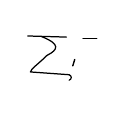
\begin{tikzpicture}[x=1pt,y=1pt,baseline=0pt,line cap=round,line join=round]
\path[use as bounding box] (0,-4) rectangle (28,18);
% Complete Sigma_i^-; joined head/body. Short dotless index retains its local recorded qualification.
\node[anchor=base west,inner sep=0pt,outer sep=0pt] at (0,0) {$\phantom{\Sigma_i^-}$};
\draw[line width=.45pt] (0,15)--(14,14.6);
\draw[line width=.45pt] (5,14.8) .. controls (12,12) and (11,10) .. (7,8) .. controls (4,5) and (1,3) .. (1,2)--(15,1) .. controls (16,.5) and (16,-.5) .. (15,-1);
\draw[line width=.5pt] (17,6.5)--(16.3,4.2);
\draw[line width=.45pt] (20,14)--(25,14);
\end{tikzpicture}
% END C024-S04
$, \unsure{de|dé|qui} definit un $U_{s_-}\subset
% BEGIN C024-S05
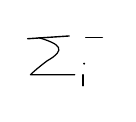
\begin{tikzpicture}[x=1pt,y=1pt,baseline=0pt,line cap=round,line join=round]
\path[use as bounding box] (0,-5) rectangle (29,19);
\node[anchor=base west,inner sep=0pt,outer sep=0pt] at (0,0) {$\phantom{\Sigma_i^-}$};
\draw[line width=.5pt] (0,15)--(15,16);
\draw[line width=.45pt] (4,15.4) .. controls (12,13) and (14,11) .. (7,7) .. controls (3,4) and (1,2) .. (1,2)--(17,2);
\draw[line width=.5pt] (20,2)--(20,-2);
\fill (20.4,6) circle (.4pt);
\draw[line width=.45pt] (21,15.5)--(27,15.5);
\end{tikzpicture}
% END C024-S05
$ tel que $\overline{U_{s_-}}\cap E_i\ne\varnothing$),
% archive sheet number: 23
